% !TEX root = SystemTemplate.tex

\chapter{Design  and Implementation}
The software is designed and implemented in term of different components, and it can be split into GUI and database. \\



\section{Database}
[DW]
 
 

\section{Major Component \#1 }


\subsection{Technologies  Used}
This section provides a list of technologies used for this component.  The details 
for the technologies have already been provided in the Overview section. 

\subsection{Component Overview}
There are several tables in database stores different information and interact with each other.\\


\subsubsection{Account table}
Store account's information of admins, teacher and students.\\
\textbf{t\_id:} foreign key which links teacher and account table together\\
\textbf{admin\_id:} foreign key which links admin and account table together\\
\textbf{name:} username\\
\textbf{password:} password\\
\textbf{access\_level:} different user's group has different access level

\subsubsection{Address table}
Store address of admins, teacher and students\\
\textbf{id:} This is a primary key and store address id.\\
\textbf{street:} Store information of street.\\
\textbf{city:} Store information of city.\\
\textbf{zipcode:} Store information of zipcode.\\
\textbf{country:} Store information of country.\\


\subsubsection{Admin table}
Store information of admins\\
\textbf{admin\_id:} Store admin's id\\
\textbf{admin\_name:} Store admin's name\\
\textbf{admin\_home\_phone:} Store admin's hone phone number\\
\textbf{admin\_cell\_phone:} Store admin's cell phone number\\
\textbf{admin\_work\_phone:} Store admin's work phone number\\
\textbf{admin\_email:} Store admin's email address\\
\textbf{admin\_sex:} Store admin's sex\\
\textbf{admin\_ssn:} Store admin's social security number\\
\textbf{admin\_pay\_rate:} Store pay rate of admin

\subsubsection{Class table}
Store classes' information\\
\textbf{class\_id:} This is a primary keystore class' id\\
\textbf{class\_name:} Store the name of class \\
\textbf{class\_time:} Store the starting time of class\\
\textbf{class\_end\_time:} Store the ending time of class\\
\textbf{class\_cost:} Store the price of the class\\
\textbf{class\_day:} Store which day has class\\
\textbf{class\_location:} Store the location of class\\
\textbf{class\_cap:} Store the capacity of class\\
\textbf{class\_clothing:} Store the clothing requirement of class\\
\textbf{class\_description:} Store the class' description\\
\textbf{class\_start\_date:} Store the start date of class\\
\textbf{class\_end\_date:} Store the end date of class\\
\textbf{class\_age:} Store the starting range of class age allowed\\
\textbf{class\_age\_end:} Store the ending range of class age allowed

\subsubsection{Guardian table}
Store guardians' information\\
\textbf{g\_id:} This is a primary key store guardian id\\
\textbf{a\_id:} This is a foreign key links guardian and address tables together\
\textbf{g\_name:} Store the name of guardian\\
\textbf{g\_phone:} Store guardian's phone number \\
\textbf{g\_work\_phone:}Store guardian's work phone number\\
\textbf{g\_email:} Store guardian's email

\subsubsection{Student table}
Store students' information\\
\textbf{stu\_id:} This is a primary key store student's id\\
\textbf{g\_id:} This is a foreign key links guardian and student tables together\\
\textbf{a\_id:} This is a foreign key links student and address tables together\\
\textbf{stu\_name:} Store student name\\
\textbf{birthday:} Store student birthday\\
\textbf{email:} Store student email\\
\textbf{daytime:} Store available time of student\\
\textbf{cellphone:} Store student cell phone number\\
\textbf{hour:}Store hours of classes student is taken\\
\textbf{tuition:} Store student unpaid tuition\\


\subsubsection{Teacher table}
Store teachers' information\\
\textbf{t\_id:}This is a primary key store teacher's id\\
\textbf{a\_id:}This is a foreign key links address and teacher tables together\\
\textbf{t\_name:} Store teacher's name\\
\textbf{home\_phone:} Store teacher's hone phone number\\
\textbf{cell\_phone:} Store teacher's cell phone number\\
\textbf{work\_phone:} Store teacher's work phone number\\
\textbf{email:} Store teacher's email address\\
\textbf{sex:} store teacher's sex\\
\textbf{ssn:} Store teacher's social security number\\
\textbf{pay\_rate:} Store teacher's pay rate\\
\textbf{medical\_information:} store teacher's medical information


\subsubsection{Student\_Class table}
Link student and class tables together\\
\textbf{stu\_id:} This is a foreign key and primary key links student and student-class tables together\\
\textbf{class\_id:} This is a foreign key and primary key links class and student-class tables together\\
\textbf{class\_finished:} Store whether student finished this class\\
\textbf{class\_approval:} Store whether student get approved for this class\\
\textbf{stu\_data\_taken:} Store when student took the class
\subsubsection{Teacher\_Class table}
Link teacher and class tables together\\
\textbf{t\_id:} This is a primary and foreign key links teacher and teacher-class together\\
\textbf{class\_id:} This is a primary and foreign key links class and teacher-class tables together


\subsection{ Architecture  Diagram}
It is important to build and maintain an architecture diagram.  However, it may 
be that a component is best described visually with a data flow diagram. 

\subsection{Phase Overview}

\subsubsection{Initial creation}
There are Student, teacher, admins and class tables and each are connected by different relationship in order to perform certain functionality we want. It consists many-to-many relationship has intermediate table and many-to-one relationship. We also have N account table for user authentication and it has permission level included in order to distinguish different user groups for example admin and teacher have different permission levels.\\

\subsubsection{Later creation}
We are going to add new table for billing and payroll in later spring.\\
(updated in spring 4)\\

\subsection{ Architecture  Diagram}
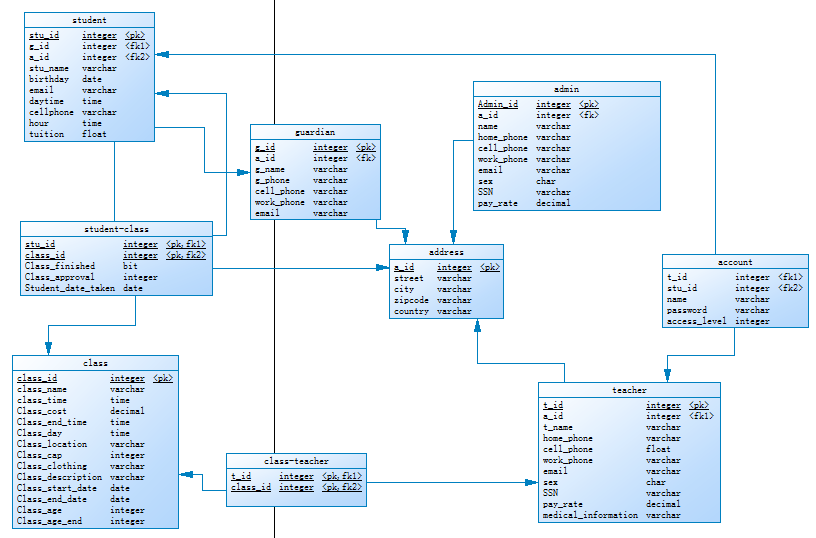
\includegraphics[scale=0.8]{pics/database.png}\\


\subsection{Data Flow Description}
Each table has different purposes for example teacher's table is for storing information of teachers and student's table's is for storing information of student. Different tables are evoked by different functionality for instance the function of search for students' information will use student and guardians and address tables at same time, and for assign teacher to classes it will use teacher and class and class-teacher table at same time


\section{GUI}
[DW]
\subsection{Technologies  Used}
We mainly use PyQt and Qt Designer for our GUI development.

\subsection{Component  Overview}
There are several components in our GUI design and can be divided into four parts authentication pages, admin pages, teacher pages and student pages.

\subsection{Phase Overview}
\subsubsection{Initial Creation}
We first created login and permission-level pages which is for authentication purposes. Then, we made two landing pages, one is for admins and another is for teachers. Those landing pages contain several sub-pages which corresponding to certain group of functionalities.
\subsubsection{Later Creation}
We are going to add a web interface for student in spring 3.5.\\
(updated in spring 3.5)\\
 
\subsubsection{authentication pages}
It consists of a login page and a permission-level page which to authenticate user and lead them to corresponding landing page.\\
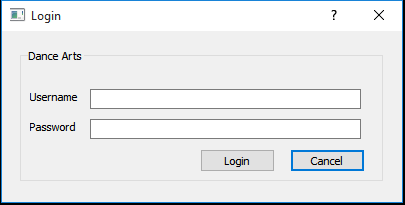
\includegraphics[scale=0.7]{pics/login_page.png}
\subsubsection{admin landing pages} 
It consists of a admin landing page and several sub-pages where admin can perform certain functionalities.\\
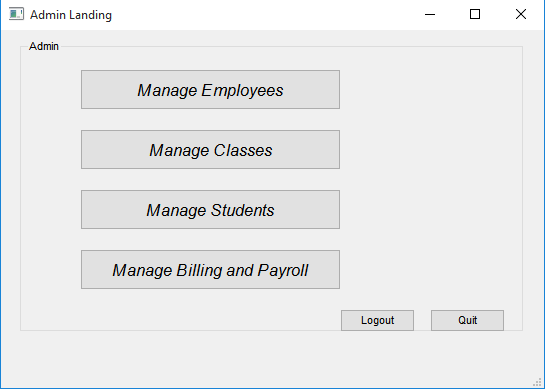
\includegraphics[scale=0.7]{pics/admin_landing.png}

\subsubsection{teacher landing pages} 
It consists of a teacher landing page and several sub-pages where teacher can perform certain functionalities.\\
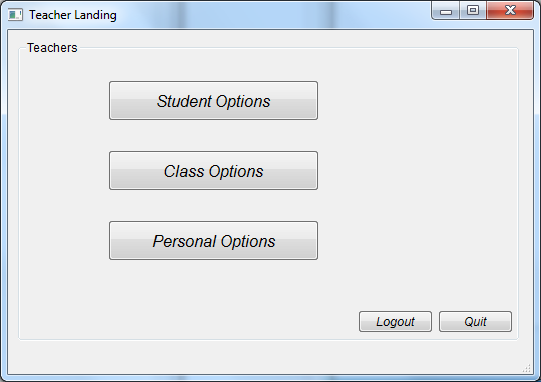
\includegraphics[scale=0.7]{pics/teacher_landing.png}

\subsubsection{student pages}
Need to update in spring 3.5

\subsection{Architecture Diagram}
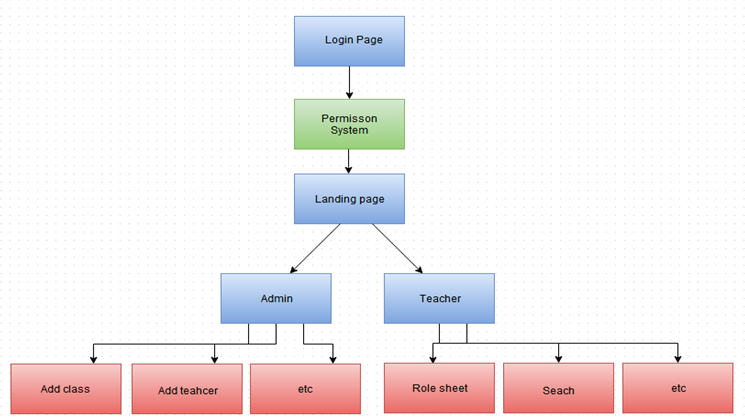
\includegraphics[scale=0.5]{pics/gui.png}\\

\subsection{Data Flow Description}
 Users can log into system through the login page and if username and password are correct then it leads user to permission system which currently is a dialogue box otherwise users get rejected from system. From permission system, user either can be leaded to admin's landing page or teacher's landing page. Then if user is admin they can search employees’ information, add class, add teacher, assign teacher to class, sets clothing requirement for specific class. If users are teachers, they can search students’ information, assign students to class, print the role sheet of the class she is teaching.
In spring 3.5, we also going to add a student web interface and they can use that to register classes and check class schedule. 

\subsection{Design Details}
<<<<<<< HEAD
\subsubsection{Role Sheet Page}
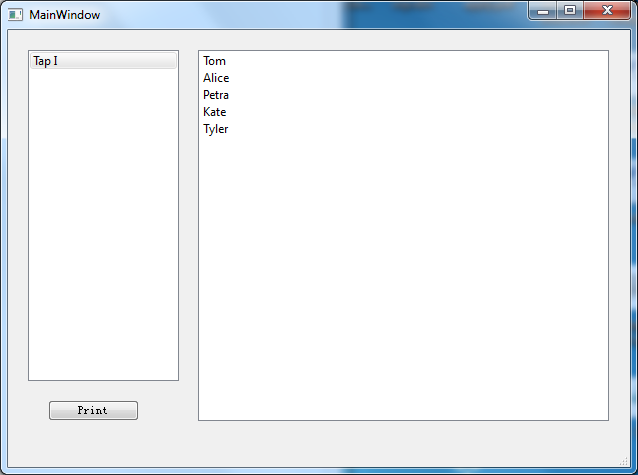
\includegraphics[scale=0.5]{pics/role.png}\\
This window provides a list of classes the teacher, who logs in to system, is currently teaching on the left list view. User can select specific class and it will populate a list of name of student those are in this class\\
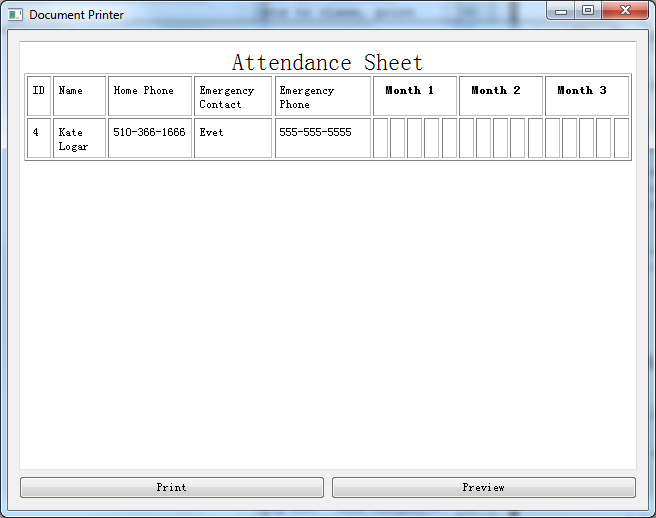
\includegraphics[scale=0.5]{pics/print.png}\\
By clicking print button, it will pop up a window which has the student's names in a text list and user can directly modify names in text list. In later spring, we are going to add some format for the list and make it looks better. User also can import external txt or xml file by clicking open button. Before print use can use preview to generate a pdf with list names of student on it and to see whether it is the list user wants to use. By clicking print button, use can print the actual list.

\subsubsection{Update Form Page}
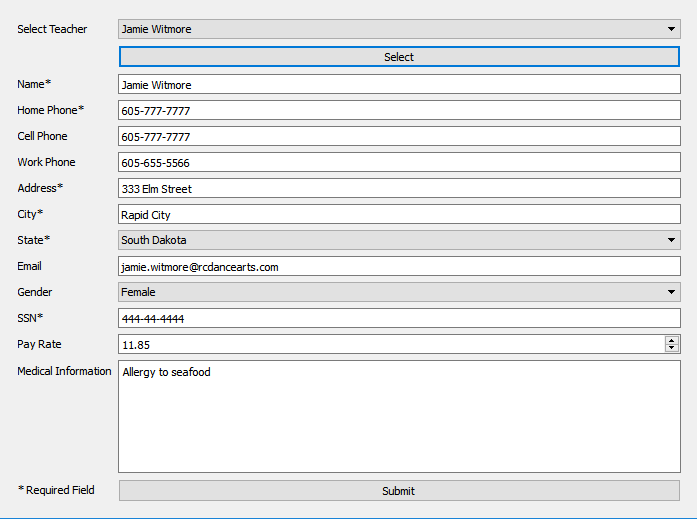
\includegraphics[scale=0.5]{pics/Update Teacher.png}\\

\subsubsection{Add Information Page}
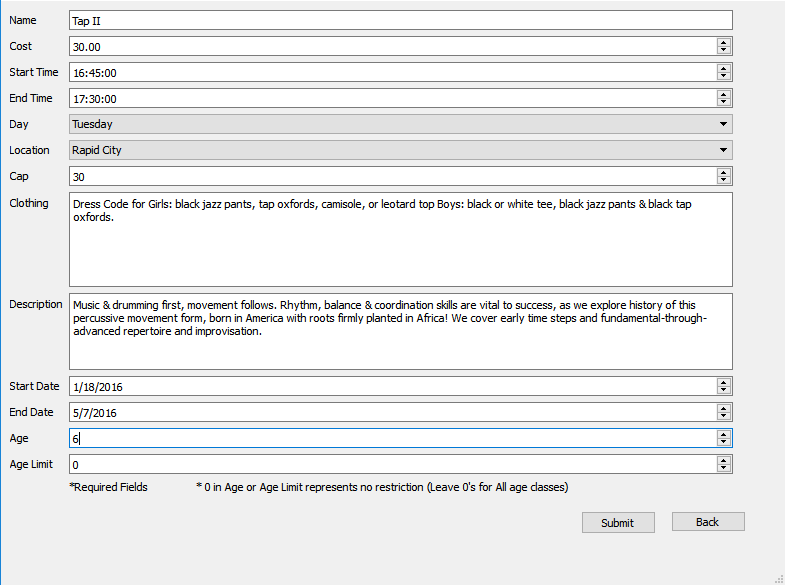
\includegraphics[scale=0.5]{pics/Add_class.png}\\
In the system there is a  multitude of different information that could be added this includes classes, teachers, and students. This is normally done in the system through the use of various forms for data entry.

The forms vary depending on the needs of the entry and will check required field when the submit button is clicked. A dialogue box will pop up asking the user to read over and finalize their entry to the database. The form then closes and the user is returns to the main page for their level.

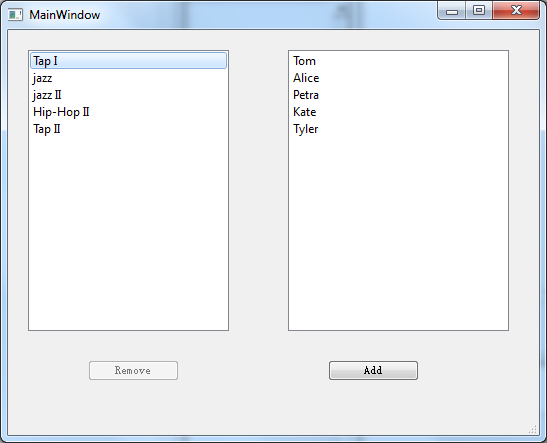
\includegraphics[scale=0.5]{pics/assin_stu.png}\\
This window provides a list of classes which studio are currently running on the left list view. By clicking certain class, it will populate a list of student's names who are in the class for the class on right list view. User can choose specific student and click remove button in order to remove student from class.
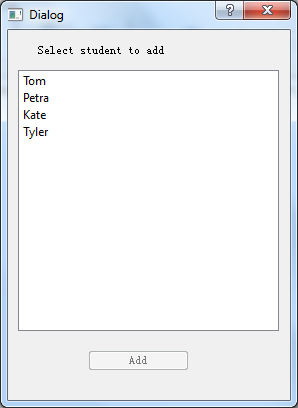
\includegraphics[scale=0.5]{pics/assin_stu_2.png}\\
clicking add button which pops up a dialog containing a list of student's names who are rejected or pending then click add button to add student.

\subsubsection{Search Page}
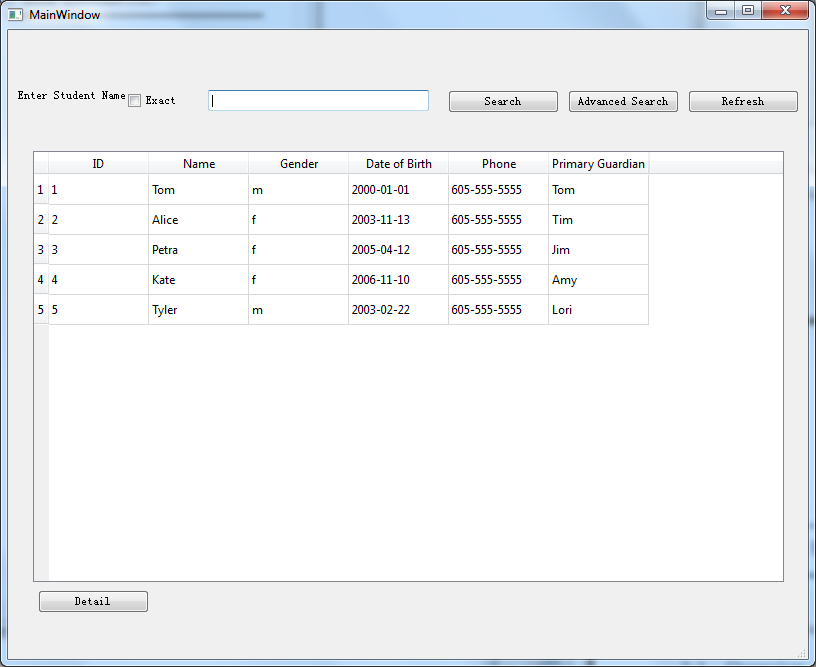
\includegraphics[scale=0.5]{pics/search.png}\\
This window provides the ability for searching information students and employees. User can search full or partial name by check or unchecked exact box, and it will populate brief information on the table view.
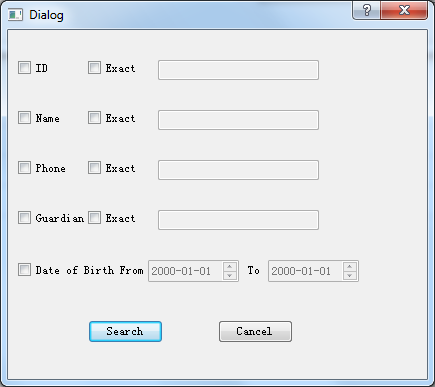
\includegraphics[scale=0.5]{pics/adv_search.png}\\
User can do advanced search by clicking advanced search button. It will let user to choose what kinds of attributes the user wants to use and do the and operation search.\\
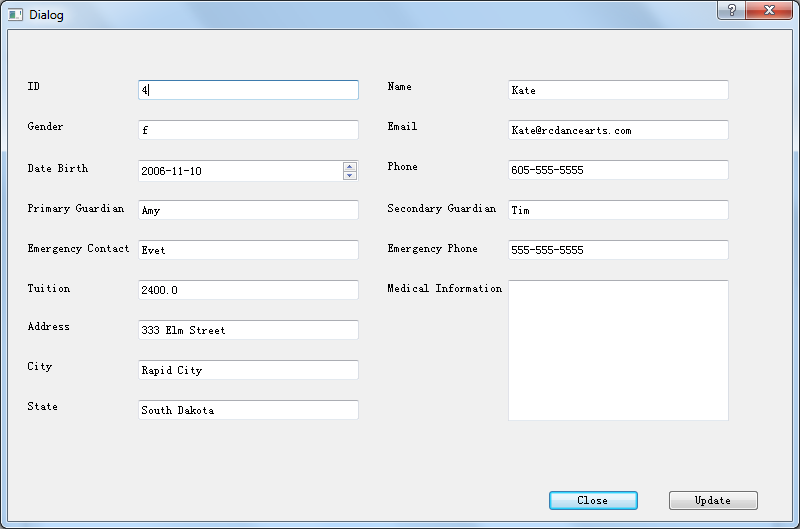
\includegraphics[scale=0.5]{pics/detail.png}\\
User can look into details of each one in the list and click detail button, it will pop up a window that shows detailed information. User also can directly modify information appears in text fields and click submit button to submit new information to database.
\subsubsection{Assign Teacher}
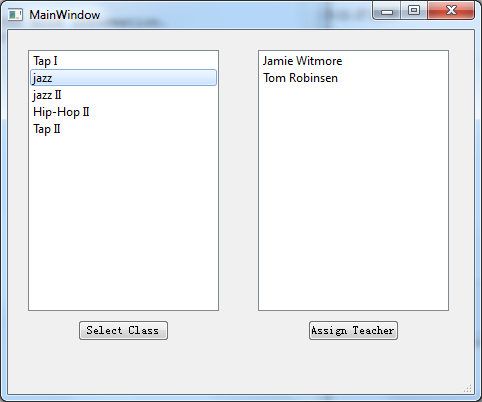
\includegraphics[scale=0.5]{pics/assign_teacher.png}\\
The assign teacher page is how a user will assign a selected teacher to a class. This is done through a window that pops up with two fields. The user will then select a class from the list of classes and a list of available teachers will appear in the right field. The user then selects a teacher and clicks yes on the confirmation message. The system then submits the SQL query to the system with the selected teacher and class. 

If the user selects a classes that is already assigned then the GUI will pop up a message telling the user who is currently assigned to teach the class. The user can then select if they want to change the teacher assigned. If the user selects yes then the right field will populate with a list of other available teachers, retrieved using a query to the database.
